\section{Technical Approach}
To infer information about Java code we use existing Java inference tools and 
combine their output. Additionally we have our own framework which allows us to
implement our own analysis. 

Most inference tools available put annotations into 
the Java class files. So does our own framework. To get the inferred information
back into the source files we use the annotation file utilities \cite{AFU} 
(TODO: How to cite a website???). 
These consist of several tools. One allows to extract annotations
from the class files. Thereby the information gets stored in an external file.
Javarifier - one of the tools which we use - directly supports to generate those
external annotation files. In a next step we use another annotation file utility which
merges the source files with the corresponding annotation files.

\begin{figure}
\centering
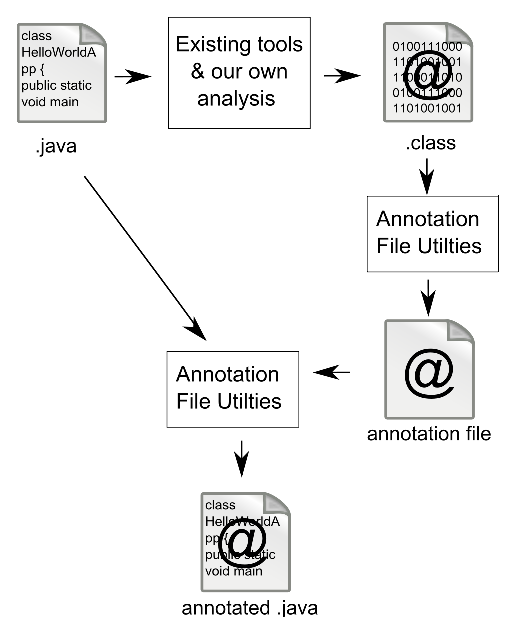
\psfig{file=figures/technicalApproach/technicalApproach.eps, width=2.1in}
\caption{Toolchain}
\end{figure}

\subsection{Analysis Framework}

To implement our own analysis tools we use the current version of the Java 7 compiler.
This allows us to use it's plugin architecture to write our own analyzers. From within
a Java compiler plugin we can access the compiler's abstract syntax tree and we can emit 
annotation to the class files. As described above those annotation will get extracted 
with the annotation file utilities.
